\documentclass[a4paper,12pt]{report}
\usepackage{multicol}
\usepackage[toc,page]{appendix}
\usepackage{amsmath}
\usepackage{float}
\usepackage{graphicx}
\usepackage{subfig}
\usepackage{amssymb}
\usepackage{geometry}
\usepackage{setspace}
\usepackage{soul}
\usepackage{dsfont}
\usepackage{multirow}% http://ctan.org/pkg/multirow
 \geometry{
 a4paper,
 total={170mm,257mm},
 left=20mm,
 top=20mm,
 }
\usepackage{tikz}
\usepackage{pgfplots}
\usetikzlibrary{shapes, arrows.meta, decorations.pathreplacing, positioning, petri, fit, calc}
\tikzstyle{startstop} = [rectangle, rounded corners, minimum width=2cm, minimum height=0.5cm,text centered, text width=3cm, draw=black, fill=gray!30]
\tikzstyle{process} = [rectangle, minimum width=2cm, minimum height=0.5cm, text centered, text width=3cm, draw=black, fill=blue!30]
\tikzstyle{detail} = [rectangle, minimum width=7cm, minimum height=0.5cm, text justified, text width=6.5cm, draw=black, fill=white!30]
\tikzstyle{smalldetail} = [rectangle, minimum width=3.5cm, minimum height=0.5cm, text justified, text width=3cm, draw=white, fill=white!30]
\tikzstyle{decision} = [rectangle, minimum width=3cm, minimum height=1cm, text centered, draw=black, fill=green!30]

\usepackage[utf8]{inputenc}

% Default fixed font does not support bold face
\DeclareFixedFont{\ttb}{T1}{txtt}{bx}{n}{10} % for bold
\DeclareFixedFont{\ttm}{T1}{txtt}{m}{n}{10}  % for normal

% Custom colors
\usepackage{color}
\definecolor{deepblue}{rgb}{0,0,0.5}
\definecolor{deepred}{rgb}{0.6,0,0}
\definecolor{deepgreen}{rgb}{0,0.5,0}

\usepackage{listings}

% Python style for highlighting
\newcommand\pythonstyle{\lstset{
language=Python,
basicstyle=\ttm,
otherkeywords={self},             % Add keywords here
keywordstyle=\ttb\color{deepblue},
emph={MyClass,__init__},          % Custom highlighting
emphstyle=\ttb\color{deepred},    % Custom highlighting style
stringstyle=\color{deepgreen},
frame=tb,                         % Any extra options here
showstringspaces=false            % 
}}


% Python environment
\lstnewenvironment{python}[1][]
{
\pythonstyle
\lstset{#1}
}
{}

% Python for external files
\newcommand\pythonexternal[2][]{{
\pythonstyle
\lstinputlisting[#1]{#2}}}

% Python for inline
\newcommand\pythoninline[1]{{\pythonstyle\lstinline!#1!}}

\begin{document}
\tableofcontents

\title{Machine Learning}
\maketitle
\part{Week 3: Classification and Logistic Regression}
\section{Logistic regression: binary classification}
\textbf{Logistic regression} is a \textbf{classification algorithm} where the value $y$ take only a small number of discrete values. 
\\
\begin{itemize}
\item \textbf{binary classification} problem: $y$ can only take 2 values: $y \in \{0,1\}$.('0' is called the negative class and '1' the positive class). Given $x^{(i)}$, the corresponding $y^{(i)}$ is also called \textbf{the label} (for the training example).
\item \textbf{multi-class classification problem}: $y \in \{0,1,2,3\}$ or more.
\end{itemize}

\subsection{Hypothesis representation}
The classifier must output value between 0 and 1: $ 0 \leq h_{\theta}(x)  \leq 1$, which can be achieved using $sigmoid$ function:

\begin{align*}
h_{\theta}(x) & = g(\theta^{\mathrm{T}} x) = \frac{1}{1+e^{- \theta^{\mathrm{T}}x}}
\end{align*}

\begin{figure}
\centering
\begin{tikzpicture}
\begin{axis}[
    axis lines = left,
    xlabel = $z$,
    ylabel = {$g(z)$},
]
%Below the red parabola is defined
\addplot [
    domain=-10:10, 
    samples=100, 
    color=red,
]{1/(1+exp(-x))};
\addplot [
    domain=-10:10, 
    samples=100, 
    color=black,
]{0.5};
\end{axis}
\end{tikzpicture}
\caption{Sigmoid (Logistic) function: $g(z) =\frac{1}{1+e^{-z}} $} \label{fig:M1}
\end{figure}




\textbf{We interpret} $h_{\theta}(x)$ \textbf{as the estimate of the probability of} $y=1$ on input $x$.

\begin{align*}
\begin{split}
 P(y=1|x;\theta) & = h_{\theta}(x) \\
 P(y=0|x;\theta) & = 1 - h_{\theta}(x) \\
 P(y=1|x;\theta) & + P(y=0|x;\theta) = 1
\end{split}
\end{align*}
$P(y=1|x;\theta)$ reads: probability that $y=1$ given $x$ parameterized by $\theta$.

\textit{Exple:} if for $x=\left[ \begin{smallmatrix} x_0 \\ x_1 \end{smallmatrix} \right] = \left[ \begin{smallmatrix} 1 \\ \mathrm{tumor\ size} \end{smallmatrix} \right]$, $h_{\theta}(x)=0.7$, it implies that there is $70\%$ chance that the tumor of the patient is malignant $(y=1)$. \\

\subsection{Decision boundary}
\begin{align*}
h_{\theta}(x) = g(\theta^{\mathrm{T}}x) =\frac{1}{1+e^{(\theta^{\mathrm{T}}x)}} = P(y=1|x;\theta)
\end{align*}
From the sigmoid curve, one can see that :
\begin{align*}
\begin{split}
\mathrm{Predict \ } y=1 & \mathrm{if\ }  h_{\theta}(x)=g(\theta^{\mathrm{T}x}) \geq 0.5 \Rightarrow \mathrm{when \ } \theta^{\mathrm{T}} x  \geq 0  \\
\mathrm{Predict \ } y=0 & \mathrm{if\ } h_{\theta}(x)=g(\theta^{\mathrm{T}x}) < 0.5 \Rightarrow\theta^{\mathrm{T}}x < 0
\end{split}
\end{align*}

\textit{Exple:} Let's assume a hypothesis function: $h_{\theta}(x) = g(\theta_0 + \theta_1 x_1 + \theta_2 x_2$, with $\theta=\left[ \begin{smallmatrix} -3\\ 1\\1 \end{smallmatrix} \right]$
\begin{figure}[H]
	\centering
        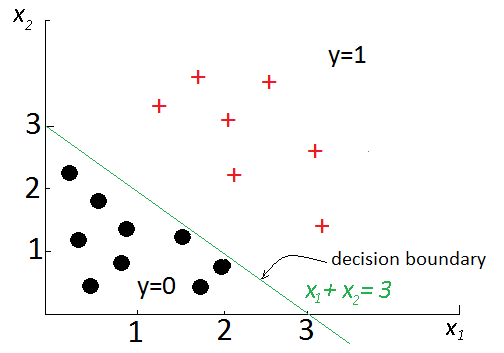
\includegraphics[totalheight=5 cm]{boundary.png}
\end{figure}
\begin{itemize}
				\item Predict $y=1$ if $\theta^{\mathrm{T}x} = -3+x_1+x_2 \geq 0 \Rightarrow (x_1+x_2) \geq 3$
				\item Predict $y=0$ if $\theta^{\mathrm{T}x} = -3+x_1+x_2 < 0 \Rightarrow (x_1+x_2) < 3$
				\end{itemize} 
The decision boundary is defined by $h_{\theta}(x) = 0.5$ ($x_1 + x_2 = 3)$	

			  
\subsection{Cost function for a classification problem}
\begin{itemize}
\item Training set: $\{(x^{(1)}, y^{(1)}), (x^{(2)}, y^{(2)}), (x^{(3)}, y^{(3)}), ........, (x^{(m)}, y^{(m)}) \}$ with $m$ examples
\item feature vector: $x = \left[ \begin{smallmatrix} x_0\\ x_1\\x_2 \\. \\. \\. \\x_n \end{smallmatrix} \right] \in \mathbb{R}^{n+1}$ with $x_0=1$, and $y \in \{0,1\}$
\item The hypothesis: $h_{\theta}(x) = \frac{1}{1 + e^{-\theta^{\mathrm{T}} x}}$
\end{itemize}
\textbf{For linear regression}, we defined the cost function $J(\theta)$:
\begin{align*}
J(\theta) = \frac{1}{m} \sum_{i=1} ^m \frac{1}{2} \left(h_{\theta}(x^{(i)}) - y^{(i)} \right)^2 =  \frac{1}{m} \sum_{i=1} ^m \mathrm{Cost}\left[h_{\theta}(x^{(i)}), y^{(i)}\right]
\end{align*}
where "Cost":
\begin{align*}
\mathrm{Cost(h_{\theta}(x),y)} = \frac{1}{2} \left(h_{\theta}(x) - y \right)^2
\end{align*}
\begin{figure}[H]
\centering
        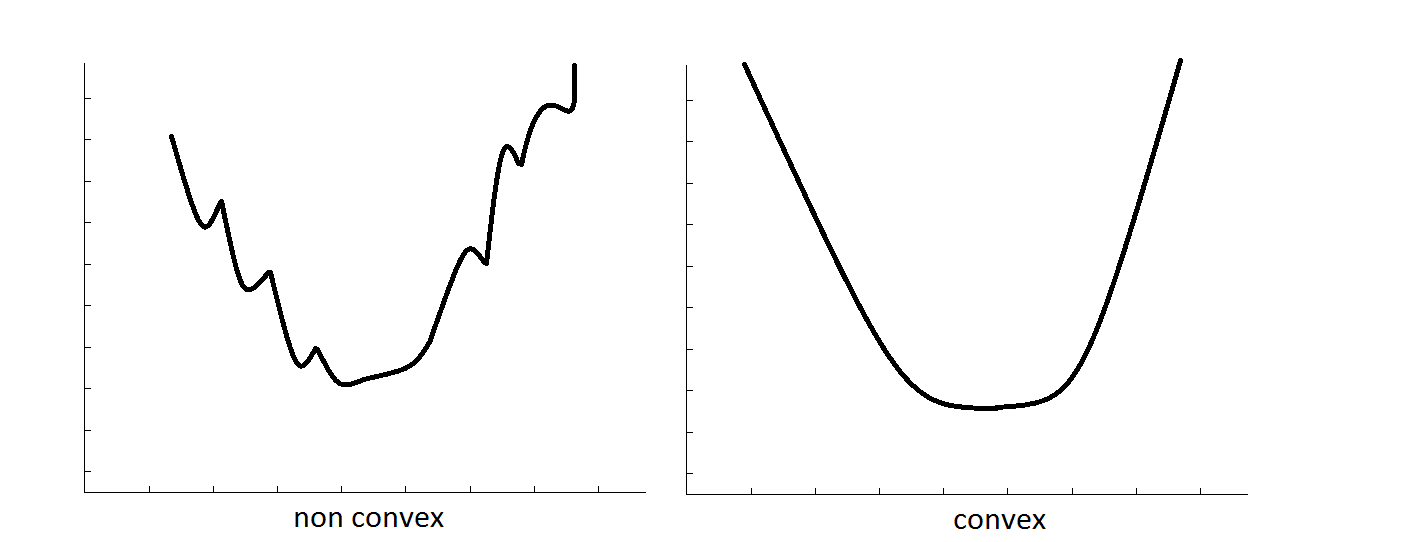
\includegraphics[totalheight=5 cm]{convec.png}
\end{figure}

For logistic regression, we use a different form of the function "Cost" and $J(\theta)$, so that $J(\theta)$ is convex, and gradient descent can converge:
\begin{align*}
\mathrm{Cost}(h_{\theta}(x), y)=
\begin{cases}
-\mathrm{Log}(h_{\theta}(x))  & \mathrm{if\ } y=1\\
-\mathrm{Log}(1-h_{\theta}(x)) & \mathrm{if\ } y=0
\end{cases}
\end{align*} 

\begin{figure}[H]
\centering
        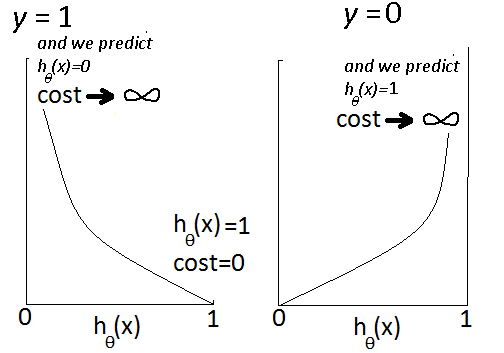
\includegraphics[totalheight=6 cm]{cost.png}
\end{figure}
The function '$\mathrm{Cost}$' can take a compact form:
\begin{align*}
\mathrm{Cost}(h_{\theta}(x), y) = -y \mathrm{Log}\left[h_{\theta}(x)\right] - (1-y)\mathrm{Log}\left[1-h_{\theta}(x)\right]
\end{align*}
If $y=1$, $\mathrm{Cost}(h_{\theta}(x),y) = -\mathrm{Log}(h_{\theta}(x))$ like in granular form of the equation. Similarly for $y=0$\\
Hence, $J(\theta)$ becomes:
\begin{align*}
\begin{split}
J(\theta) & = \frac{1}{m} \sum_{i=1} ^m \mathrm{Cost}(h_{\theta}(x^{(i)}), y^{(i)}) \\
& = -\frac{1}{m} \left(\sum_{i=1} ^m y^{(i)}\mathrm{Log}(h_{\theta}(x^{(i)})) + (1-y^{(i)})\mathrm{Log}\left[1-h_{\theta}(x^{(i)})) \right] \right)
\end{split}
\end{align*}

\subsection{Gradient Descent}
\begin{enumerate}
\item Make prediction given $x$ $\Rightarrow$ output: $h_{\theta}(x) = \frac{1}{1+e^{-\theta^{\mathrm{T}}x}} = h_{\theta}(x) = P(y=1|x;\theta)$
\item Calculate the cost function $J(\theta)$
\item Similarly to Batch Gradient Descent, we need $\mathrm{min}_{\theta} J(\theta)$. \\
\noindent\rule{\linewidth}{0.4pt} 
\\ \textit{Repeat until convergence} \{
\begin{align*}
\theta_j  := \theta_j - \alpha \frac{\partial}{\partial \theta_j} J(\theta)\\
\end{align*}
with
\begin{align*}
\frac{\partial}{\partial \theta_j} J(\theta) = \frac{1}{m} \sum_{i=1} ^m \left(h_{\theta}(x^{(i)})-y^{(i)}\right) x_j ^{(i)}
\end{align*}
(update all $\theta_j$ simultaneously: $j = 0$ to $n$)\\
\} \\
\noindent\rule{\linewidth}{0.4pt}
\end{enumerate}

\textbf{Note that feature scaling can also be applied to logistic regression}
\section{Advanced Optimization}
There are several optimization algorithms:
\begin{align*}
\begin{array}{ll}
    \bullet \ \mathrm{Gradient \ Descent} \\
		\left.
		\begin{array}{ll}
					\bullet \ \mathrm{conjugate \  gradient}\\
					\bullet \ \mathrm{BFGS}\\
					\bullet \ \mathrm{L-BFGS}
		\end{array}
		\right\} \parbox{4cm}{\tiny{No need to manually pick $\alpha$. Faster than Gradient descent. But, they are also more complex.}}
\end{array}
\end{align*}
(*advanced Numerical Computing *)

In MatLab, \textbf{\textit{fminunc()}} (function minimization unconstrained) is a built-in advanced optimization function ($>>$ help \textbf{\textit{fminunc}}). In Python, the package \textbf{\textit{scipy.optimize}} includes some optimization algorithms:


Here is the procedure for using \textit{\textbf{fminunc()}}:

\begin{enumerate}
	\item Step1: Generate a function \textit{\textbf{costFunction}} that outputs 2 arguments
			\begin{itemize}
				\item \textit{jVal}: the value of $J(\theta)$
				\item \textit{gradient}: a vector with the value of the gradients
			\end{itemize}
\begin{python}
function [jVal, gradient] = costFunction(theta)
	jVal = [' code to compute J(theta) ']; 
	gradient = zeros(n+1, 1) #create a zero vector 
	#and fill with gradient values 
	gradient(1) = [' code to compute (d J(theta)/d theta_0) ']; 
	gradient(2) = [' code to compute (d J(theta)/d theta_1)	'];
	.....
	.....
	gradient(n+1) = [' code to compute (d J(theta)/d theta_(n))	'];			
\end{python}

\item Step2: Set the options
\begin{python}
options = optimset('GradObj', 'on', 'MaxIter', '100');
\end{python}
\begin{itemize}
\item '100' is the maximum number of iterations
\item 'GradObj', 'on' : tells \textbf{\textit{fminunc()}} that our function returns both the cost and the gradient  
\end{itemize}
Initial guess for theta \\
\begin{python}
initialtheta = zeros(n+1,1)
\end{python}
\item Step3: run \textit{\textbf{fminunc()}}
\begin{python}
[optTheta, functionVal, exitFlag] = fminunc(@CostFunction, initialTheta, options)
\end{python}
'@CostFunction' is a pointer to the function \textbf{\textit{CostFunction()}}.
\item Setp 4: \textbf{\textit{fminunc()}} outputs 3 parameters values:
\begin{itemize}
\item \textbf{optTheta} = optimum value of $\theta$ as a vector
\item \textbf{functionVal} ($\approx 0$) is the costFuntion value at optimum
\item \textbf{exitFlag} (=1) shows convergence status. 
\end{itemize}
\end{enumerate}



\section{Multiclass classification}
Example of multiclass classification: email foldering/tagging \\
\begin{align*}
\begin{matrix} & \mathrm{work} & \mathrm{friends} & \mathrm{family} & \mathrm{hobby} \\
											& y=1 & y=2 & y=3 & y=4 \\
										\mathrm{or} \rightarrow & y=0 & y=1 & y=2 & y=4	
\end{matrix}
\end{align*}
\begin{table}[!htb]
\centering
\begin{tabular}{c|c}
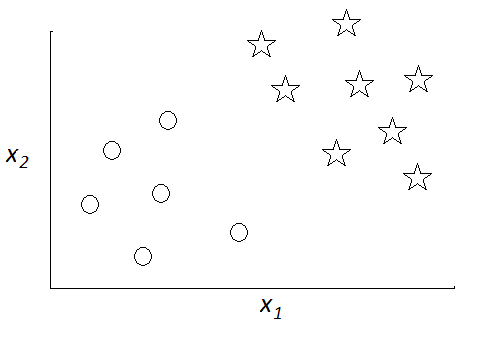
\includegraphics[width=5cm]{class2.png} &
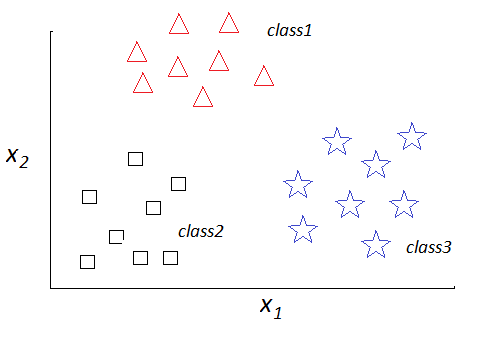
\includegraphics[width=5cm]{multiclass.png} \\
\textbf{\begin{footnotesize}Binary Classification\end{footnotesize}} & \textbf{\begin{footnotesize}Multiclass classification\end{footnotesize}}
\end{tabular}
\end{table}

\subsection{One-vs-all (one-vs-rest) classification}
Transform a multiclass ($k$) problem into several ($k$) binary classes problems

Principle: Train a logistic regression classifier $h_{\theta}^{(i)} (x)$ for each class $i$ to predict the probability that $y=i$.\\
On a new input $x$, to make a prediction, pick the class $i$ that maximizes $h_{\theta}^{(i)}(x)$ $\Rightarrow$ $\mathrm{max}_{i} h_{\theta}^{(i)}(x)$.\\
Run all three classifier on input $x$ and then choose classifier given the larger value ($max_{i} h_{\theta}^{(i)}(x)$.
\begin{table}[!htb]
\centering
\begin{tabular}{c|c}
 & 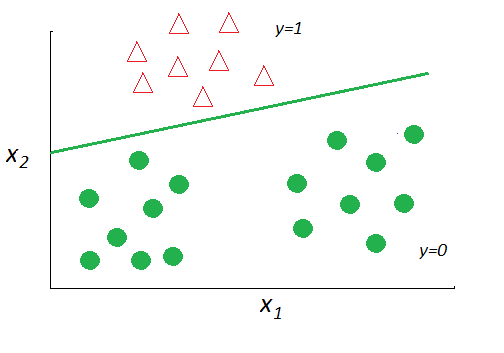
\includegraphics[width=4cm]{multiclassh1.png}
\tiny{Classifier $h_{\theta} ^{(1)}(x)$- class 1 is positive class}
 \\
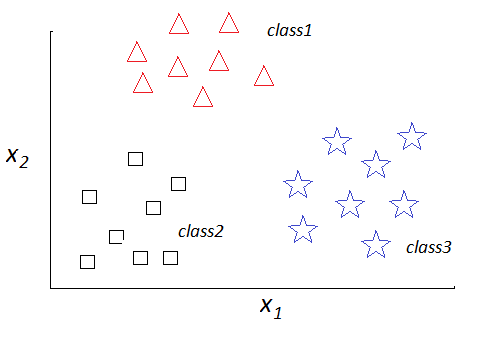
\includegraphics[width=5cm]{multiclass.png} & 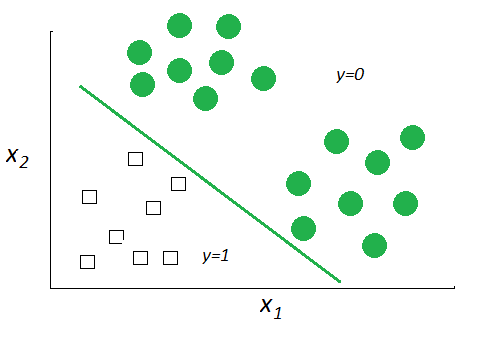
\includegraphics[width=4cm]{multiclassh2.png}
\tiny{Classifier $h_{\theta} ^{(2)}(x)$- class 2 is positive class} \\
& 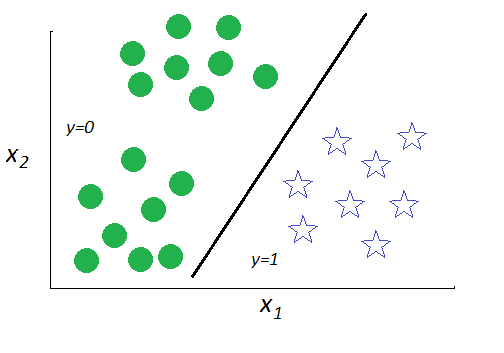
\includegraphics[width=4cm]{multiclassh3.png}
\tiny{Classifier $h_{\theta} ^{(3)}(x)$- class 3 is positive class}
\end{tabular}
\end{table}
\begin{align*}
h_{\theta}^{(i)} (x) = P(y=i|x;\theta) \mathrm{with\  i=1,2,3}
\end{align*}

\section{Underfitting(bias), Overfitting(variance)}
\begin{table}[h]
\centering
\begin{tabular}{ccc}
 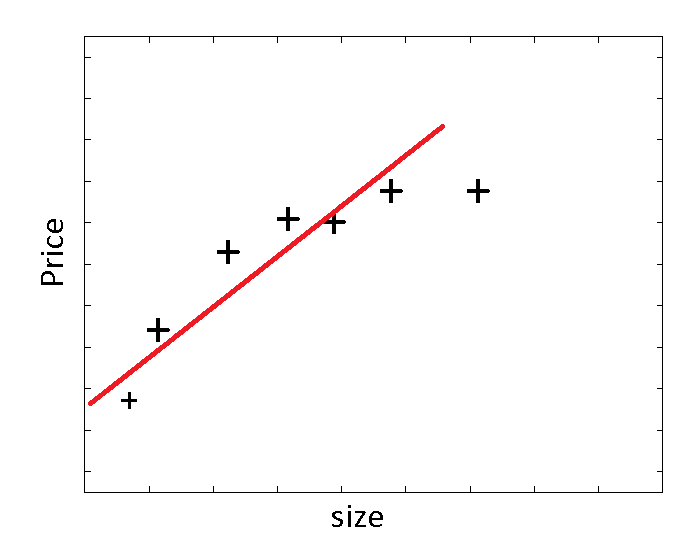
\includegraphics[width=4cm]{underfitting.png} & 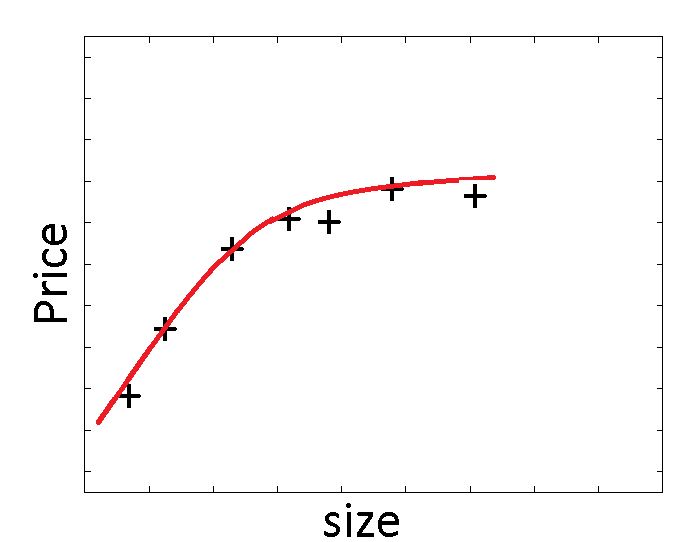
\includegraphics[width=4cm]{goodfitting.png} & 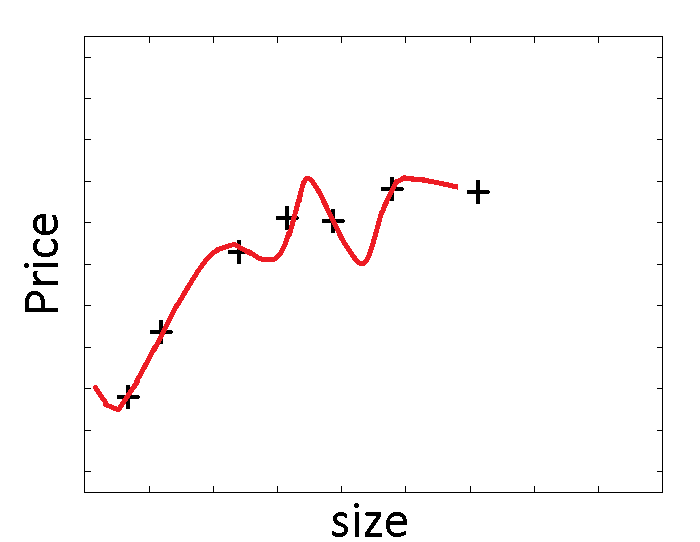
\includegraphics[width=4cm]{overfitting.png} \\
\tiny{$h_{\theta}(x) = \theta_0 + \theta_1 x$} & \tiny{$h_{\theta}(x) = \theta_0 + \theta_1 x + \theta_2  x^2$} & \tiny{$h_{\theta}(x) = \theta_0 + \theta_1 x + \theta_2  x^2 + \theta_3 x^3 + \theta_4 x^4$} \\
\parbox{4cm}{\tiny \textbf{Underfitting/High Bias}. There is a high bias of the model to fit the data to a linear despite the trend.} & &\parbox{4cm}{\tiny \textbf{Overfitting/High Variance}. There are too many features. The algorithm makes accurate predictions in the training example ($J(\theta)=0)$, but fails to generalize to new examples}
\end{tabular}
\end{table}

Bias/Variance also apply to logistic regression. \\ \\

\textbf{How to adress overfitting :}
\begin{itemize}
	\item Option1: 
	\begin{itemize}
		\item Reduce the number of features (select the more important features manually)
		\item Model selection algorithm
	\end{itemize}
	
	\item Option2: Regularization $\Rightarrow $ keep all the features but reduce magnitude of $\theta_j$
\end{itemize}


\subsection{Regularization}
The goal is to reduce the values/amplitudes of the parameters $\theta_j$ (with $j=$1,2...n), to mitigate overfitting (overconfidence). Often overfitting si associated with very large coefficients $\theta$
\begin{figure}[H]
\centering
        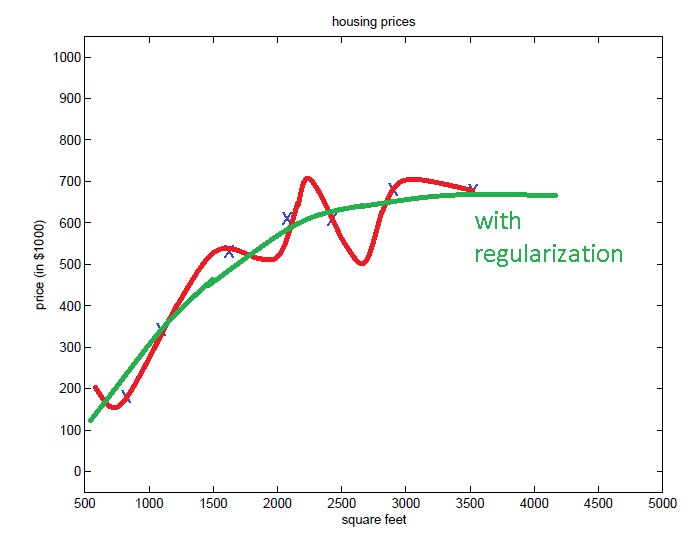
\includegraphics[totalheight=6 cm]{overfittingregularization.png}
\end{figure}
\begin{itemize}
\item There are several options for the regularization term
	\begin{itemize}
		\item sum of squares ($L_2$ norm):
		\begin{align}
		|| \ theta ||_2 = \sum _{j=1} ^{n} \theta_j ^2
		\end{align}
				\item sum of absolute values ($L_1$ norm):
		\begin{align}
		|| \theta ||_1 = \sum _{j=1} ^{n} |\theta_j|
		\end{align}
	\end{itemize}
\end{itemize}


\begin{itemize}
\item Features: $\left[\begin{smallmatrix} x_0 \\ x_1 \\..\\..\\..\\x_n \end{smallmatrix} \right]$
\item Parameters: $\left[\begin{smallmatrix} \theta_0 \\ \theta_1 \\..\\..\\..\\\theta_n \end{smallmatrix} \right]$
\end{itemize}
\begin{align*}
J(\theta) = \frac{1}{2m} \left[ \sum_{i=1} ^m \left( h_{\theta}(x^{(i)}) - y^{(i)} \right)^2 + \lambda \sum_{j=1} ^{n} \theta_j ^2\right]
\end{align*}
$\lambda$ is the regularization parameter. By convention, $\theta_0$ is excluded from the regularization.\\
If \textbf{$\lambda$ is too large} ($\lambda = 10^{10}$), algorithm would result in \textbf{underfitting} (fails to fit even the training set): $(\theta_1,\theta_2,\theta_3...)$  parameters would be too much penalized $\approx 0$ $\Rightarrow$ $\theta_1x^{(1)} \approx \theta_2 x^{(2)}... \approx 0$ and hence $h_{\theta}(x) = \theta_0$.
\\ \\
\subsubsection{Regularized linear regression}
\begin{itemize}
\item Cost function
\begin{align*}
J(\theta) = \frac{1}{2m} \left[ \sum_{i=1} ^m \left( h_{\theta}(x^{(i)}) - y^{(i)} \right)^2 + \lambda \sum_{j=1} ^{n} \theta_j ^2\right]
\end{align*}
($\theta_0$ is excluded from the regularization term: $j=1...n$).
\item Gradient descent: $\mathrm{min}_{\theta} J(\theta)$ with $h_{\theta}(x) = \theta^{\mathrm{T}}x$ \\
\end{itemize}

\noindent\rule{\linewidth}{0.4pt} 
\\ \textit{Repeat until convergence} \{
\begin{align*}
\begin{split}
\theta_0  &:= \theta_0 - \alpha\frac{1}{m} \sum_{i=1} ^{m} \left( h_{\theta}(x^{(i)})-y^{(i)}\right) x_{0}^{(i)}\\
... & ...\\
... & ...\\
\theta_j  &:= \theta_j - \alpha\frac{1}{m} \sum_{i=1} ^{m} \left( h_{\theta}(x^{(i)})-y^{(i)}\right) x_{j}^{(i)} + \frac{\lambda}{m} \theta_j\\
\mathrm{for \ }  &  j=1,2,3...n
\end{split}
\end{align*}
\} \\
\noindent\rule{\linewidth}{0.4pt}
The equation of $\theta_j$ can be simplified:
\begin{align*}
\theta_j  := \theta_j\left(1- \alpha\frac{\lambda}{m} \right) - \alpha\frac{1}{m} \sum_{i=1} ^{m} \left( h_{\theta}(x^{(i)})-y^{(i)}\right) x_{j}^{(i)} \\
\end{align*}

\subsubsection{Normal equation}
With $X \in \mathbb{R}^{m \times (n+1)} $ and $y\in \mathbb{R}^{m}$

\begin{align*}
\mathrm{without \ regularization:\ } & \theta = \left(X^{\mathrm{T}}X \right)^{-1} X^{\mathrm{T}} y\\
 \mathrm{with \ regularization:\ } & \theta = \left(X^{\mathrm{T}}X + \lambda \left[\begin{smallmatrix} 0&0&0&0...&0\\0&1&0&0...&0\\0&0&1&0...&0\\.&.&.&...&.\\.&.&.&...&.\\.&.&.&...&.\\0&0&0&0..&1 \end{smallmatrix} \right]\right)^{-1} X^{\mathrm{T}} y 
\end{align*}
The matrix of (zeros and ones) is a $(n+1) \times (n+1)$. \\ \\

\textbf{Non-invertibility:} \\
Suppose $m \leq n$ (\# exples $\leq$ \#features), then $(X^{\mathrm{T}}X)$ will be singular/non-invertible/degenerate (although MatLab can still provide a pseudo-inverse with '\textbf{\textit{pinv()}}'.
\\
If $\lambda > 0$, then $(X^{\mathrm{T}}X + \lambda M)$ -where $M$ is the special matrix- is invertible: regularization makes the matrix invertible.

\subsubsection{Regularized logistic Regression}
\begin{itemize}
\item Cost function $J(\theta)$:\\
\begin{align*}
J(\theta) = - \frac{1}{m} \left[ \sum_{i=1} ^m y^{(i)} \mathrm{Log} ( h_{\theta}(x^{(i)})) + (1- y^{(i)}) \mathrm{Log} ( 1- h_{\theta}(x^{(i)})) \right] + \frac{\lambda}{2m} \sum_{j=1} ^{n} \theta_j ^2
\end{align*}

\item Gradient descent: $h_{\theta}(x) = \frac{1}{1+e^{-\theta^{\mathrm{T}}x}}$ \\
\noindent\rule{\linewidth}{0.4pt} 
\\ \textit{Repeat until convergence} \{
\begin{align*}
\begin{split}
\theta_0  &:= \theta_0 - \alpha\frac{1}{m} \sum_{i=1} ^{m} \left( h_{\theta}(x^{(i)})-y^{(i)}\right) x_{0}^{(i)}\\
\theta_j  &:= \theta_j - \alpha\frac{1}{m} \sum_{i=1} ^{m} \left( h_{\theta}(x^{(i)})-y^{(i)}\right) x_{j}^{(i)} + \frac{\lambda}{m} \theta_j\\
....& j=1,2,3...n
\end{split}
\end{align*}
\} \\
\noindent\rule{\linewidth}{0.4pt}
\end{itemize}

\textbf{With Advanced Optimization}: \\
\begin{python}
function [jVal, gradient] = costFunction(theta)
	jVal = [' code to compute J(theta) ']; 
	gradient = zeros(n+1, 1) #create a zero vector 
	#and fill with gradient values 
	gradient(1) = [' code to compute (d J(theta)/d theta_0) ']; 
	gradient(2) = [' code to compute (d J(theta)/d theta_1)	'];
	.....
	.....
	gradient(n+1) = [' code to compute (d J(theta)/d theta_(n))	'];			
\end{python}
where:

\begin{align*}
J(\theta) & = \left[ -\frac{1}{m} \sum_{i=1} ^m y^{(i)} \mathrm{Log} \left(h_{\theta}(x^{(i)}) \right) + (1-y^{(i)}) \mathrm{Log} \left(1-h_{\theta}(x^{(i)}) \right) \right] + \frac{\lambda}{2m} \sum_{j=1} ^{n} \theta_j ^2 \\
\frac{\partial}{\partial \theta_0}J(\theta) & = \frac{1}{m} \sum_{i=1} ^m \left(h_{\theta}(x^{(i)}) - y^{(i)} \right) x_0 ^{(i)} \\
\frac{\partial}{\partial \theta_1}J(\theta) & = \left[ \frac{1}{m} \sum_{i=1} ^m \left(h_{\theta}(x^{(i)}) -y^{(i)} \right) x_1 ^{(i)} \right] + \frac{\lambda}{m} \theta_1 \\
\end{align*}

\section{Assignments}
\subsection{Visualizing the data}
\begin{python}
function plotData(X, y)
	figure;  # Create New Figure
	hold on;
	# X is the array [x0,x1,x2] of the m training examples
	#find indexes of training examples where y=1 (positive)
	pos = find(y==1);
	#find indexes of training examples where y=0 (negative)
	neg = find(y==0); 

	m = length(y); #number of training examples
	# k+ = black plus, ko=black circles
	# MarkerSize= 7
	# Linewidth=2
	#MarkerFaceColor=yellow (filled circles)
	plot(X(pos,1), X(pos,2), 'k+', 'LineWidth', 2, 'MarkerSize', 7);
	plot(X(neg,1), X(neg,2), 'ko', 'MarkerFaceColor', 'y', 'MarkerSize', 7);
end
\end{python}
\subsection{Create the sigmoid() function}
\begin{python}
function g = sigmoid(z)
	# return g the sigmoid of z
	# z can be a vector, a matrix or a scalar
	g = zeros(size(z)); 
	#Take the exponential of z and add 1
	# 1./(...) do an inverse element wise.
	g = 1./(1 + exp(-z))
end
\end{python}
\subsection{cost function and gradient}
The cost function in logistic regression is defined by:
\begin{align*}
J(\theta) = \frac{1}{m} \sum_{i=1} ^{m} \left[-y^{(i)} \mathrm{Log}\left(h_{\theta}(x^{i})\right) - (1- y^{(i)}) \mathrm{Log}\left(1-h_{\theta}(x^{i})\right) \right]
\end{align*}
and the gradient (a vector of same length as $\theta$ where $j=0,...,n$.
\begin{align*}
\frac{\partial J(\theta)}{\partial \theta} = \frac{1}{m} \sum_{i=1} ^{m} \left( h_{\theta}(x^{i}) - y^{(i)}\right) x_j ^{(i)}
\end{align*}
\begin{python}
function [J, grad] = costFunction(theta, X, y)
	m = length(y); # number of training examples
	J = 0; #initial value of cost function
	grad = zeros(size(theta)); #initial matrix for gradient
	#co is the item inside the sum of J
	#h(x) = sigmoid(X*theta)
	co = (-y.*log(sigmoid(X*theta)))-(1-y).*log(1-sigmoid(X*theta)); 
	J = 1/m * sum(co) # J is a scalar
	#grad is a vector matrix with X'=transpose(X)
	grad = 1/m*X'*(sigmoid(X*theta) - y) 
end
\end{python}
\subsection{Plot the decision boundary}
\begin{python}
function plotDecisionBoundary(theta, X, y)
%PLOTDECISIONBOUNDARY Plots the data points X and y into a new figure with
%the decision boundary defined by theta
%   PLOTDECISIONBOUNDARY(theta, X,y) plots the data points with + for the 
%   positive examples and o for the negative examples. X is assumed to be 
%   a either 
%   1) Mx3 matrix, where the first column is an all-ones column for the 
%      intercept.
%   2) MxN, N>3 matrix, where the first column is all-ones

% Plot Data
plotData(X(:,2:3), y);
hold on

if size(X, 2) <= 3
    % Only need 2 points to define a line, so choose two endpoints
    plot_x = [min(X(:,2))-2,  max(X(:,2))+2];

    % Calculate the decision boundary line
    plot_y = (-1./theta(3)).*(theta(2).*plot_x + theta(1));

    % Plot, and adjust axes for better viewing
    plot(plot_x, plot_y)
    
    % Legend, specific for the exercise
    legend('Admitted', 'Not admitted', 'Decision Boundary')
    axis([30, 100, 30, 100])
else
    % Here is the grid range
    u = linspace(-1, 1.5, 50);
    v = linspace(-1, 1.5, 50);

    z = zeros(length(u), length(v));
    % Evaluate z = theta*x over the grid
    for i = 1:length(u)
        for j = 1:length(v)
            z(i,j) = mapFeature(u(i), v(j))*theta;
        end
    end
    z = z'; % important to transpose z before calling contour

    % Plot z = 0
    % Notice you need to specify the range [0, 0]
    contour(u, v, z, [0, 0], 'LineWidth', 2)
end
hold off

end

\end{python}

\subsection{Predict label }
This function will predict the label (0 or 1) of based on the learned logistic regression parameters theta.
\begin{python}
function p = predict(theta, X)
m = size(X, 1); # Number of training examples
p = zeros(m, 1);

# calculate sigmoid for all examples p is a vector matrix of size mx1
p = sigmoid(X*theta); 
for student = 1:m
    if p(student) >= 0.5
        p(student)=1;
    else
        p(student)=0;
    end
end
\end{python}

\subsection{Learning parameters using \textit{fminunc()}}
\begin{python}
#initialization
#clear the variables, close all figs, clc=clear command window
clear ; close all; clc 

# Load Data : col1=exam1, col2=exam2, col3=label(1 or 0)
data = load('ex2data1.txt');
X = data(:, [1, 2]); y = data(:, 3);

# ==================== Part 1: Plotting ====================
fprintf(['Plotting data with + indicating (y = 1) examples ...
and o indicating (y = 0) examples.\n']);
plotData(X, y);
#retains plots in the current axes so that 
#new plots added to the axes do not delete existing plots
hold on; 
# Labels and Legend
xlabel('Exam 1 score')
ylabel('Exam 2 score')
legend('Admitted', 'Not admitted')
hold off;

# ============ Part 2: Compute Cost and Gradient ============
# Setup the data matrix appropriately, and add ones for the intercept term
[m, n] = size(X);
#Add intercept term to x and X_test
X = [ones(m, 1) X];

# Initialize fitting parameters
initial_theta = zeros(n + 1, 1);

# Compute and display initial cost and gradient
[cost, grad] = costFunction(initial_theta, X, y);

fprintf('Cost at initial theta (zeros): \%f\n', cost);
fprintf('Gradient at initial theta (zeros): \n');
fprintf(' \%f \n', grad);

# ============= Part 3: Optimizing using fminunc  =============
#  Set options for fminunc
options = optimset('GradObj', 'on', 'MaxIter', 100);

# Run fminunc to obtain the optimal theta
#\@(t) creates a function with argument t which calls the costFunction
[theta, cost, exit_flag] = fminunc(@(t)(costFunction(t, X, y)), ...
initial\_theta, options);

% Print theta to screen
fprintf('Cost at theta found by fminunc: \%f\n', cost);
fprintf('theta: \n');
fprintf(' \%f \n', theta);

# Plot Boundary
plotDecisionBoundary(theta, X, y);
hold on;
xlabel('Exam 1 score')
ylabel('Exam 2 score')
legend('Admitted', 'Not admitted')

#============== Part 4: Predict and Accuracies: predict() ==============
#  After learning the parameters, you'll like to use it to predict the outcomes
#  on unseen data. In this part, you will use the logistic regression model
#  to predict the probability that a student with score 45 on exam 1 and 
#  score 85 on exam 2 will be admitted.

prob = sigmoid([1 45 85] * theta);
fprintf(['For a student with scores 45 and 85, we predict an admission ' ...
         'probability of %f\n\n'], prob);
# Compute accuracy on our training set
p = predict(theta, X);

fprintf('Train Accuracy: \%f\n', mean(double(p == y)) * 100);

\end{python}
\begin{figure}[H]
\centering
        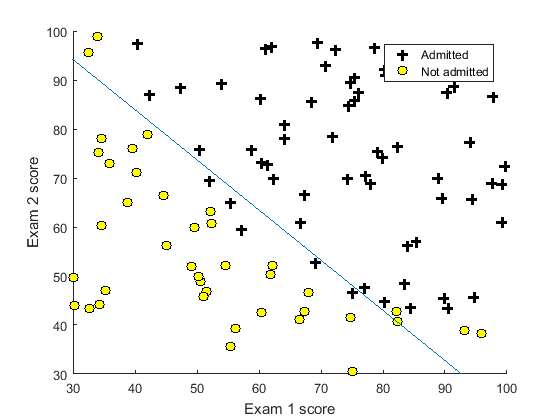
\includegraphics[totalheight=4 cm]{ex2.png}
				\caption{
				\label{} Training data with precision boundary}
\end{figure}

\begin{appendices}
\section{Logistic Regression - University of Washington Coursera}
We define $l(\theta)$ as the likelihood of $\theta$: it is a measure of the quality of the fit of the model to the training examples. Maximizing the likelihood over all possible $\theta$ will ensure to give the best classifier. For example, for 1 data, we pick a $\theta$ value that maximizes $p(y=+1|x,\theta) = \frac{1}{1+e^{-\theta^T x}}$.
\begin{itemize}
\item For $m$ examples, the likelihood is the product of the probability (assuming that the examples are independent of each other):
\begin{align*}
l(\theta) = \prod_{i=1} ^m p(y^{(i)}|x^{(i)},\theta)
\end{align*}
\end{itemize}

In order to simplify the mathematics, w use $\mathrm{Log} l(\theta)$ (the Log does not change the maxima), hence:
\begin{align*}
\mathrm{Log}(l(\theta)) = \sum_{i=1} ^m \mathrm{Log}(p(y^{(i)}|x^{(i)},\theta))
\end{align*}
We introduce the indicator function:
\begin{align}
\mathds{1}(y^{(1)}=+1)
	\begin{cases}
	+1 \mathrm{\ if \ } y^{(1)}  \\
	-1  \mathrm{\ if \ } y^{(1)} = -1
	\end{cases}
\end{align}

For one example:
\begin{align}
\begin{split}
\mathrm{Log}(l(\theta)) &= \mathds{1}(y^{(1)}=+1) P(y^{(1)}=+1|x^{(i)},\theta) + \mathbb{1}(y^{(1)}=-1) P(y^{(1)}=-1|x^{(i)},\theta) \\
&= \mathds{1}(y^{(1)}=+1) P(y^{(1)}=+1|x^{(i)},\theta) + \mathds{1}(y^{(1)}=-1) (1-P(y^{(1)}=+1|x^{(i)},\theta) \\
&=\mathds{1}(y^{(1)}=+1) P(y^{(1)}=+1|x^{(i)},\theta) + \mathds{1}(y^{(1)}=-1) \mathrm{Log}\left(1-\frac{1}{1+e^{-\theta^T x}} \right) \\
&=\mathds{1}(y^{(1)}=+1) P(y^{(1)}=+1|x^{(i)},\theta) + \mathds{1}(y^{(1)}=-1) \mathrm{Log}\left(\frac{1 + e^{-\theta^T x} -1}{1+e^{-\theta^T x}} \right) \\
&=\mathds{1}(y^{(1)}=+1) P(y^{(1)}=+1|x^{(i)},\theta) + \mathds{1}(y^{(1)}=-1) \mathrm{Log}\left(\frac{e^{-\theta^T x}}{1+e^{-\theta^T x}} \right) \\
\end{split}
\end{align}

\begin{itemize}
\item Gradient:
\end{itemize}
\begin{align}
\begin{split}
\frac{\partial{\mathrm{Log}}}{\partial \theta_j} &= -(1-\mathds{1}(y^{(1)}=+1) \frac{\partial \theta^T x}{\partial \theta_j} - \frac{\partial}{\partial \theta_j} \mathrm{Log}\left(1-e^{-\theta^T x} \right) \\
&= -(1-\mathds{1}(y^{(1)}=+1) x_j - \frac{-\theta_j e^{-\theta^T x}}{1-e^{-\theta^T x}}) \\
&=-(1-\mathds{1}(y^{(1)}=+1) x_j + x_j P(y^{(1)}=-1|x,\theta ) )\\
&=x_j \left( \mathds{1}(y^{(1)}=+1) - P(y^{(1)}=+1|x,\theta) \right)\\
\end{split}
\end{align}

For all examples $m$:
\begin{align}
\frac{\partial{\mathrm{Log}}}{\partial \theta_j} = \sum_{i=1} ^{N} x_j \left( \mathds{1}(y^{(1)}=+1) - P(y^{(1)}=+1|x,\theta \right)
\end{align}
\end{appendices}
\end{document}